\subsection{Programmierbeispiel}
\label{subsec:programmierbeispiel}
Das Programmierbeispiel welches im Folgenden dargestellt wird, erzeugt ein Fenster mit dem Titel 
\emph{Meine erste Qt App}. Zudem ein Label welches \emph{Hello World} anzeigt und ein Button mit der
Aufschrift \emph{Exit}. Sobald der Button wird, schließt sich das Fenster.

\lstinputlisting[language=C++,caption={Qt Hello World Sourcecode},
    label=lst:qtHelloWorldSourceCode]{\srcloc/StandDerTechnik/qtHelloWorld.cpp}

Daraus ergibt sich das folgende Programm
\begin{figure}[h]
    \centering
    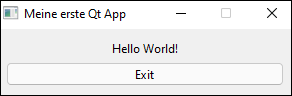
\includegraphics[width=0.5\textwidth, center]{StandDerTechnik/qtHelloWorldApp1}
    \caption[Qt Hello World App]{Qt Hello World App}
    \label{img:qtHelloWorldApp}
\end{figure}